
%(BEGIN_QUESTION)
% Copyright 2013, Tony R. Kuphaldt, released under the Creative Commons Attribution License (v 1.0)
% This means you may do almost anything with this work of mine, so long as you give me proper credit

Suppose a Rosemount model 3244MV (FOUNDATION Fieldbus) transmitter is used as a voltage sensor for a solar panel, the transmitter configured to sense DC millivolt input and connected to a voltage divider network to reduce the solar panel's voltage down to a level the 3244MV transmitter can handle:

$$\includegraphics[width=15.5cm]{i03382x01.eps}$$

Determine the proper {\tt XD\_Scale}, {\tt OUT\_Scale}, and {\tt L\_Type} parameter values to make the transmitter functional over the solar array's expected voltage range of 0 to 29 volts.

\underbar{file i03382}
%(END_QUESTION)





%(BEGIN_ANSWER)

{\tt L\_Type} = Indirect

\vskip 10pt

{\tt XD\_Scale} = 0 to 96.67 mV

\vskip 10pt

{\tt OUT\_Scale} = 0 to 29 volts

%(END_ANSWER)





%(BEGIN_NOTES)

{\bf This question is intended for exams only and not worksheets!}.

%(END_NOTES)


